\documentclass[10pt,twocolumn,letterpaper]{article}
\usepackage[pagenumbers]{cvpr}
\usepackage{multirow}
\definecolor{cvprblue}{rgb}{0.21,0.49,0.74}
\usepackage[breaklinks,colorlinks,allcolors=cvprblue]{hyperref}
\def\confName{CS 412}
\def\confYear{2026}

\title{Do Network Intrusion Detectors Generalize?\\A Cross-Dataset Comparison of Machine Learning Models\\[4pt]\large Intermediate Project Report}

\author{Daniel Kolawole\\
University of Illinois Chicago\\
CS 412 Introduction to Machine Learning, Fall 2026}

\begin{document}
\maketitle

\begin{abstract}
Machine learning intrusion detectors often report F1 scores above 0.95, but those scores usually come from training and testing on the same dataset. This project checks what happens when a detector trained on one network is tested on a different network. So far, three public NetFlow datasets that share the same 43 features have been sampled and cleaned, and logistic regression, a random forest, and a multilayer perceptron have been trained and tested on every combination of training and test dataset. All three models reach an average in-dataset F1 of at least 0.93. On networks they were not trained on, their average F1 drops to between 0.05 and 0.19. The random forest scores the best in-dataset and transfers the worst.
\end{abstract}

\section{Introduction and Problem Description}

A network intrusion detection system, or NIDS, watches traffic on a network and flags connections that look like attacks. Machine learning fits this task well because a model can learn what attack traffic looks like from labeled examples instead of relying on hand written rules. Many papers report very high scores for these models, often above 99 percent accuracy. Even so, machine learning detectors are still rarely trusted in real networks.

Sommer and Paxson argued that intrusion detection is harder for machine learning than most tasks because attacks are rare, normal traffic changes a lot from one network to another, and mistakes are expensive \cite{sommer2010}. Arp \etal later reviewed 30 papers from the top security conferences and found that sampling bias was at least partly present in 90 percent of them \cite{arp2022}. A big part of the problem is how detectors are tested. Most papers split one dataset at random into a training set and a test set. The test flows then come from the same lab, the same attack tools, and the same time period as the training flows. A detector can score well in that setup by learning the quirks of one lab network instead of the general behavior of attacks.

This project asks how well an intrusion detector trained on one network works on a network it has never seen, and whether the type of model changes how much performance drops. The proposal also added two follow-up questions. The first is whether training on more than one network helps a model generalize. The second is which flow features each model depends on and whether those features carry the same meaning across networks.

Testing across networks used to be hard because every public dataset had its own feature format. Sarhan, Layeghy, and Portmann fixed this by converting several well known datasets into one shared set of 43 NetFlow features \cite{sarhan2022}. Their follow-up work tested whether a shared feature set helps models generalize and used SHAP values to explain which features the models relied on \cite{sarhan2022bdr}. This project builds on that work by running a full train-on-one, test-on-another comparison across several model families from this course. Every model uses the same samples, splits, preprocessing, and metrics, so the differences between models are easy to compare.

This is a solo project, so all of the work in this report was done by Daniel Kolawole.

\section{Data}

The project uses three datasets from the NetFlow v2 collection released by the University of Queensland \cite{sarhan2022}. Each one is a NetFlow version of an older, well known dataset, so all three share the same 43 features and the same binary label. Table~\ref{tab:data} lists them. They were picked because they come from very different environments. UNSW-NB15 was generated in the UNSW Canberra cyber range in 2015 \cite{moustafa2015}. CSE-CIC-IDS2018 was built on Amazon Web Services by the Canadian Institute for Cybersecurity to look like an enterprise network \cite{sharafaldin2018}. ToN-IoT comes from a testbed built around Internet of Things and industrial devices \cite{moustafa2021}. NF-BoT-IoT-v2 was left out because 99.64 percent of its flows are attacks, which makes a benign versus attack comparison hard to read.

\begin{table}[t]
\centering
\small
\begin{tabular}{lrrrr}
\toprule
Dataset & Flows & Attack \% & Classes & Sample \\
\midrule
UNSW-NB15 & 2,390,275 & 3.98 & 9 & 299,798 \\
ToN-IoT & 16,940,496 & 63.99 & 9 & 300,587 \\
CIC-IDS2018 & 18,893,708 & 11.95 & 14 & 300,519 \\
\bottomrule
\end{tabular}
\caption{The three NetFlow v2 datasets. Flows and attack share are for the full datasets. Classes counts the attack types, not including benign. Sample is the number of flows kept for this project.}
\label{tab:data}
\end{table}

The three datasets differ a lot in class balance, and that matters for evaluation. Attacks make up about 4 percent of UNSW-NB15, 12 percent of CIC-IDS2018, and 64 percent of ToN-IoT. The attacks themselves are different too. The largest attack class is exploits in UNSW-NB15, scanning in ToN-IoT, and the HOIC DDoS attack in CIC-IDS2018.

The full datasets have between 2.4 million and 18.9 million flows, which is too many to train dozens of models on with limited compute. Each dataset was read in chunks and a random sample of about 300,000 flows was kept, using a fixed random seed. The sample keeps the original class balance, as Table~\ref{tab:data} shows. Keeping the real balance is important because precision and false positive rate both depend on how rare attacks are \cite{arp2022}.

Five columns were removed before training. These are the source and destination IP addresses, the source and destination ports, and DNS\_QUERY\_ID. IP addresses and ports point to specific machines in each lab, so a model could memorize them instead of learning what attacks look like. Arp \etal call this a spurious correlation \cite{arp2022}. DNS\_QUERY\_ID is a random transaction number, so it should not carry any real signal. The proposal also planned to drop timestamps, but the v2 datasets do not include timestamp columns, so nothing had to be removed there. This leaves 38 numeric features. They cover byte and packet counts, flow duration, TCP flags, TTL values, packet size bins, throughput, and a few protocol fields like the DNS query type and the FTP return code.

\section{Work Done So Far}

\subsection{Data pipeline and preprocessing}

Each 300,000 flow sample was split into 70 percent training, 15 percent validation, and 15 percent test data. The split is stratified by label and uses a fixed seed, which gives about 210,000 training flows and 45,000 flows each for validation and testing. The test sets are fixed and shared by every experiment. Because of this, an in-dataset result and a cross-dataset result are always measured on exactly the same test flows.

Most NetFlow features are counts with very long tails. In the UNSW-NB15 sample, for example, the median number of incoming bytes in a flow is 1,580 but the largest value is over 30 million. Every feature is transformed with \mbox{$\log(1+x)$} and then standardized. The standardization is fit only on the training data of the dataset the model is trained on. When the model is tested on a different dataset, that dataset is transformed with the same fitted values, which is how a deployed model would see new traffic. Standardized values are clipped to the range from $-10$ to $10$ so a few extreme flows cannot dominate.

\subsection{Models}

Three models are done so far. The first is logistic regression from scikit-learn, trained with the L-BFGS solver for up to 2,000 iterations. The second is a random forest with 100 trees and at least 2 samples per leaf. The third is a multilayer perceptron written in PyTorch with two hidden layers of 128 and 64 units, ReLU activations, and dropout of 0.1. It is trained with Adam at a learning rate of 0.001 and a batch size of 1,024 for up to 30 epochs. Training stops early when the validation loss does not improve for 3 epochs, and the weights from the best epoch are kept. This connects to the course topics on logistic regression, deep learning, and backpropagation.

Every model is trained with three random seeds, and the tables report the mean. Logistic regression gives the same result for every seed, so its spread is zero. All models use a fixed decision threshold of 0.5. The threshold is never tuned on test data, since tuning it on the test set would give inflated results \cite{arp2022}.

\subsection{Evaluation}

Each model is trained on one dataset and tested on the test split of all three datasets. This gives a 3 by 3 grid for each model. The diagonal of the grid is the usual in-dataset setting, and the six off-diagonal cells are cross-dataset tests. The metrics are recall on the attack class, which is the detection rate, false positive rate, precision, F1 on the attack class, and ROC AUC. Accuracy is recorded too, but only to show how misleading it can be when classes are imbalanced. The generalization gap of a model is its average in-dataset F1 minus its average cross-dataset F1.

\subsection{Preliminary results}

\begin{figure*}[t]
\centering
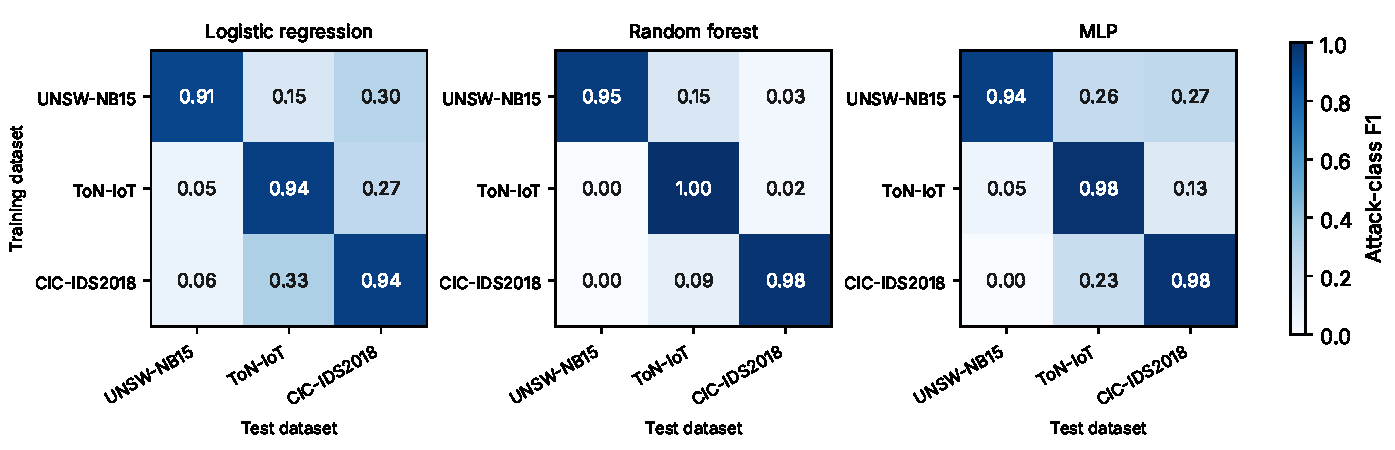
\includegraphics[width=0.92\linewidth]{f1_matrix.pdf}
\caption{Attack-class F1 for every pair of training and test dataset, averaged over three seeds. The diagonal is the in-dataset result. Every off-diagonal cell is a model tested on a network it never saw during training.}
\label{fig:matrix}
\end{figure*}

\begin{table*}[t]
\centering
\small
\begin{tabular}{lcccccccc}
\toprule
& \multicolumn{3}{c}{F1} & \multicolumn{2}{c}{ROC AUC} & \multicolumn{3}{c}{Cross-dataset} \\
\cmidrule(lr){2-4}\cmidrule(lr){5-6}\cmidrule(lr){7-9}
Model & In-dataset & Cross-dataset & Gap & In-dataset & Cross-dataset & Recall & FPR & Accuracy \\
\midrule
Logistic regression & 0.930 & 0.194 & 0.736 & 0.963 & 0.614 & 0.442 & 0.400 & 0.469 \\
Random forest & 0.977 & 0.049 & 0.928 & 0.996 & 0.413 & 0.037 & 0.144 & 0.649 \\
MLP & 0.968 & 0.157 & 0.811 & 0.995 & 0.493 & 0.285 & 0.314 & 0.527 \\
\bottomrule
\end{tabular}
\caption{In-dataset results are averaged over the three diagonal cells and cross-dataset results over the six off-diagonal cells, each with three seeds. The gap is in-dataset F1 minus cross-dataset F1.}
\label{tab:summary}
\end{table*}

Figure~\ref{fig:matrix} shows the main result so far. Every model does well on its own dataset, with in-dataset F1 between 0.91 and 0.995. The scores fall apart as soon as the test data comes from another network. Averaged over the six cross-dataset pairs, F1 is 0.194 for logistic regression, 0.157 for the MLP, and 0.049 for the random forest. Table~\ref{tab:summary} gives the summary numbers.

The ranking of the models flips between the two settings. The random forest is the best model in-dataset, with an average F1 of 0.977 and an average AUC of 0.996. It is also the worst model across datasets, with an average cross-dataset AUC of 0.413. An AUC under 0.5 means the model ranks benign flows as more suspicious than attacks, so on the new network it does worse than random guessing. Logistic regression is the simplest model and has the smallest gap. This supports the hypothesis from the proposal that more complex models would score higher in-dataset without generalizing better. Logistic regression is still nowhere near usable across networks, though.

The models also fail in different ways. Some flag almost everything. Logistic regression trained on ToN-IoT flags 93.7 percent of the benign UNSW-NB15 flows as attacks. Others miss almost everything. The random forest trained on CIC-IDS2018 gets an F1 of 0.000 on UNSW-NB15 but an accuracy of 96.0 percent, because it labels nearly every flow benign and about 96 percent of UNSW-NB15 is benign. This is the exact case where accuracy hides a detector that catches nothing \cite{arp2022}.

Cross-dataset results are also much less stable than in-dataset results. In-dataset F1 changes by less than 0.005 between seeds. The random forest trained on UNSW-NB15 and tested on ToN-IoT gets an F1 of 0.077, 0.329, and 0.047 for the three seeds. A small change in how the trees are built changes a lot when the test data looks nothing like the training data.

\section{What Remains}

The next step is the self-attention model from the proposal, based on the FT-Transformer design \cite{gorishniy2021}. Each feature becomes a token, a small transformer encoder mixes the tokens, and a classification token makes the prediction. Training this model on the CPU is much slower than the MLP, so it will be trained on a smaller subsample of each training set. To keep the comparison fair, the MLP will also be retrained on the same subsample.

The second remaining experiment is multi-source training. Each model will be trained on two datasets combined and tested on the third one. This checks whether more varied training data closes the gap or only shrinks it.

The third remaining part is the feature analysis. Permutation importance will show which features each model depends on, and comparing the distribution of those features across the three datasets will show whether they mean the same thing on every network. If time allows, the stretch goal from the proposal is a benign-only autoencoder that flags flows it cannot reconstruct well.

After that, the remaining work is the final presentation on November 25, the final report due December 1, and putting the code on GitHub as the project instructions require.

{
\small
\bibliographystyle{ieeenat_fullname}
\bibliography{refs}
}

\end{document}
